%%Template made by Uday Khankhoje for examinations using the exam template
%%Refer to the documentation http://www-math.mit.edu/~psh/exam/examdoc.pdf
%%for lot more bells and whistles to the standard template shown below
\documentclass[a4paper,11pt,addpoints]{exam}
\usepackage[left=1.5cm,right=1.5cm,top=1.5cm,bottom=2cm]{geometry}
%\usepackage{mathrsfs}
\usepackage{graphicx,color}
\usepackage[x11names]{xcolor}
\usepackage{venndiagram}
\usepackage{tikz}
\usepackage{tkz-fct}
\usepackage{tkz-euclide}
\usepackage{epic,eepic}
%\usepackage{mathpazo}
\usepackage{url}
\usepackage{tasks} % cria lista curta
\usepackage{multicol}
\usepackage{pgfplots}
\usepackage{amsmath, amsthm, amssymb}
\pointsinmargin
\boxedpoints
\renewcommand*\half{.5}
\usepackage{setspace}
\DeclareMathOperator{\vecc}{vec}

\pgfplotsset{compat=1.18, width=7cm}
%\renewcommand{\vec}[1]{\ensuremath{\mathbf{#1}}}

\global\vbadness=1616

\begin{document}
\noindent
%%PART 1 of header
\begin{center}
	\vspace*{-3em}
	\def\arraystretch{2.0}
	\begin{tabular}{|p{0.7\linewidth}|p{0.2\linewidth}|}
		\hline
		\textbf{Avaliação de Matemática - Quarto Bimestre}                                                            & Pontos Obtidos $\downarrow$ \\
		\hline
		Data:\hspace{3cm}  Total de questões \textbf{\numquestions} \hspace{1cm} Total de pontos: \textbf{\numpoints} &                             \\
		\hline
		\multicolumn{2}{|l|}{Tuma: \hspace{0.3\linewidth} Nome: \hspace{0.3\linewidth} Duração: 1 hr}                                               \\
		\hline
	\end{tabular}
\end{center}
%%PART 2 of header, if you have too many questions, this may be a problem
%%if so, use \multirowgradetable{n}[questions], where n is the number of rows you want
%%or, switch to \gradetable[h][pages] instead,
\begin{center}
	\gradetable[h][questions]
\end{center}
%%PART 3 of header
\textbf{Instruções
	\begin{enumerate}
		\item Necessário todos os cálculos.
		\item Questões de múltipla escolha sem cálculos serão desconsideradas.
	\end{enumerate}
}
%%toggle comment on next line to show/hide the answers
% \printanswers
%%Now the actual paper!
\begin{questions}

	\question[1]

	A expressão que define a função quadrática f(x), cujo gráfico está esboçado
	é:

	\begin{multicols}{2}
		\begin{tasks}
			\task $f(x) = -2x^2 -2x + 4$
			\task $f(x) = x^2 + 2x - 4$
			\task $f(x) = x^2 + x - 2$
			\task $f(x) = 2x^2 + 2x - 4$
			\task $f(x) = 2x^2 + 2x - 2$
		\end{tasks}

		\begin{center}
			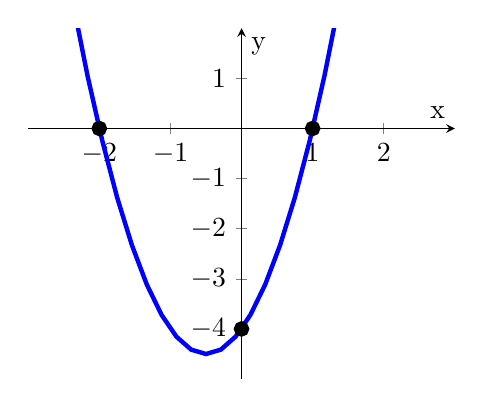
\begin{tikzpicture}
				\begin{axis}[
						every axis plot/.append style={ultra thick},
						xmin=-3,
						xmax=3,
						ymin=-5,
						ymax=2,
						axis lines=center,
						xlabel=x,
						ylabel=y,
						xtick={-2,-1,0,1,2},
						ytick={-4,-3,-2,-1,0,1}
					]
					\addplot[color=blue, domain=-3:2]{2*(x-1)*(x+2)};
					\addplot[only marks] table {
							-2 0
							1 0
							0 -4
						};
				\end{axis}
			\end{tikzpicture}
		\end{center}
	\end{multicols}

	\question[1]

	Esboce o gráfico da função quadrática $f(x) = x^2 - 2x - 8$

	\question[1]

	Esboce o gráfico da função quadrática $f(x) = x^2 - 5x + 4$

	\question[1]

	Determine os zeros ou raízes da função $f(x) = x^2 - 2x - 3$

	\question[1]

	Determine os zeros ou raízes da função $f(x) = x^2 + 10x + 25$

	\question[1]

	Determine o vértice da função quadrática $f(x) = -10x^2 - 20x - 40$

	\question[1]

	Determine o vértice da função quadrática $f(x) = x^2 - 4x - 2$

	\question[1]

	Se $f(x) = -3x^2 + 2x - 5$, quanto vale $f(-2)$?

	\question[1]

	Se $f(x) = x^2 - 3x + 1$, quanto vale $f(2)$?

	\question[1]

	Se $f(x) = 2x^2 + 3x + 4$, quanto vale $f(-5)$?

\end{questions}
\end{document}
